\documentclass[fontsize=12pt]{article}
\usepackage[english,ngerman]{babel}
\usepackage[T1]{fontenc}
\usepackage[utf8]{inputenc}
\usepackage{amsmath,amssymb}
\usepackage[colorlinks=true,linkcolor=black,anchorcolor=black,citecolor=black,filecolor=black,menucolor=black,runcolor=black,urlcolor=black]{hyperref}
\usepackage{graphicx}
\usepackage{fancyhdr}
\usepackage{lastpage}
\usepackage{pgfplots}
\usepackage{datetime2}
\usepackage{tikz}
\usepackage{pdfpages}
\usepackage{csquotes}
\usetikzlibrary{arrows.meta,patterns}
\usepackage{acronym}
\usepackage[nottoc,numbib]{tocbibind}
\usepackage{hhline}
\usepackage{eurosym}
\usetikzlibrary{ipe} % ipe compatibility library
\usepackage[backend=biber,style=apa]{biblatex}
\bibliography{bibliography.bib}

\usepackage{geometry}
 \geometry{
 a4paper,
 left=35mm,
 right=25mm,
 top=20mm,
 bottom=20mm
 }

\renewcommand{\baselinestretch}{1.5}

\renewcommand{\listoffigures}{\begingroup
\tocsection
\tocfile{\listfigurename}{lof}
\endgroup}

\renewcommand{\listoftables}{\begingroup
\tocsection
\tocfile{\listtablename}{lot}
\endgroup}

\graphicspath{{./pictures/}}
\setlength\parindent{0pt}

\tikzstyle{ipe stylesheet} = [
  ipe import,
  even odd rule,
  line join=round,
  line cap=butt,
  ipe pen normal/.style={line width=0.4},
  ipe pen heavier/.style={line width=0.8},
  ipe pen fat/.style={line width=1.2},
  ipe pen ultrafat/.style={line width=2},
  ipe pen normal,
  ipe mark normal/.style={ipe mark scale=3},
  ipe mark large/.style={ipe mark scale=5},
  ipe mark small/.style={ipe mark scale=2},
  ipe mark tiny/.style={ipe mark scale=1.1},
  ipe mark normal,
  /pgf/arrow keys/.cd,
  ipe arrow normal/.style={scale=7},
  ipe arrow large/.style={scale=10},
  ipe arrow small/.style={scale=5},
  ipe arrow tiny/.style={scale=3},
  ipe arrow normal,
  /tikz/.cd,
  ipe arrows, % update arrows
  <->/.tip = ipe normal,
  ipe dash normal/.style={dash pattern=},
  ipe dash dotted/.style={dash pattern=on 1bp off 3bp},
  ipe dash dashed/.style={dash pattern=on 4bp off 4bp},
  ipe dash dash dotted/.style={dash pattern=on 4bp off 2bp on 1bp off 2bp},
  ipe dash dash dot dotted/.style={dash pattern=on 4bp off 2bp on 1bp off 2bp on 1bp off 2bp},
  ipe dash normal,
  ipe node/.append style={font=\normalsize},
  ipe stretch normal/.style={ipe node stretch=1},
  ipe stretch normal,
  ipe opacity 10/.style={opacity=0.1},
  ipe opacity 30/.style={opacity=0.3},
  ipe opacity 50/.style={opacity=0.5},
  ipe opacity 75/.style={opacity=0.75},
  ipe opacity opaque/.style={opacity=1},
  ipe opacity opaque,
]

\definecolor{red}{rgb}{1,0,0}
\definecolor{blue}{rgb}{0,0,1}
\definecolor{green}{rgb}{0,1,0}
\definecolor{yellow}{rgb}{1,1,0}
\definecolor{orange}{rgb}{1,0.647,0}
\definecolor{gold}{rgb}{1,0.843,0}
\definecolor{purple}{rgb}{0.627,0.125,0.941}
\definecolor{gray}{rgb}{0.745,0.745,0.745}
\definecolor{brown}{rgb}{0.647,0.165,0.165}
\definecolor{navy}{rgb}{0,0,0.502}
\definecolor{pink}{rgb}{1,0.753,0.796}
\definecolor{seagreen}{rgb}{0.18,0.545,0.341}
\definecolor{turquoise}{rgb}{0.251,0.878,0.816}
\definecolor{violet}{rgb}{0.933,0.51,0.933}
\definecolor{darkblue}{rgb}{0,0,0.545}
\definecolor{darkcyan}{rgb}{0,0.545,0.545}
\definecolor{darkgray}{rgb}{0.663,0.663,0.663}
\definecolor{darkgreen}{rgb}{0,0.392,0}
\definecolor{darkmagenta}{rgb}{0.545,0,0.545}
\definecolor{darkorange}{rgb}{1,0.549,0}
\definecolor{darkred}{rgb}{0.545,0,0}
\definecolor{lightblue}{rgb}{0.678,0.847,0.902}
\definecolor{lightcyan}{rgb}{0.878,1,1}
\definecolor{lightgray}{rgb}{0.827,0.827,0.827}
\definecolor{lightgreen}{rgb}{0.565,0.933,0.565}
\definecolor{lightyellow}{rgb}{1,1,0.878}
\definecolor{black}{rgb}{0,0,0}
\definecolor{white}{rgb}{1,1,1}

\pagestyle{fancy}
\fancyhf{}
\lfoot{B. Blacher, F. Weissenbacher}
\lhead{Modellauto mit Sensorik}
\rhead{
\includegraphics[scale=0.5]{htllogo.png}}
\rfoot{\thepage{}}
 
\begin{document}
\begin{titlepage}
	\centering
	\hspace{1.5cm}
	
\includegraphics[scale=2]{htllogo.png}
	\newline
	{\huge Diplomarbeit \par}
	{\Large Fachbereich Mechatronik\par}
	\vspace{1.5cm}
	{\huge Modellauto mit Sensorik\par}
	\vspace{2cm}
	{\Large verfasst und vorgelegt von\par}
	{\huge Benjamin Blacher\par}
	{\huge Florian Weissenbacher\par}
	\vfill
	betreut von\par
	Dipl. Ing. Wolfgang \textsc{Czernin}\par
	Dipl. Ing. Matthias \textsc{Dirl}

	\vfill

	{\large Kapfenberg, \today\par}
\end{titlepage}
\newpage

%Tikz example
%\begin{figure}[h]
%\centering
%\begin{tikzpicture}[ipe stylesheet]
%%content
%\end{tikzpicture}
%\caption{Sender-Empfänger-Modell}
%\label{fig:SenderEmpfaenger}
%\end{figure}

%section example
%\section{xxx}
%\label{sec:xxx}

%subsection example
%\subsection{xxx}}
%\label{subsec:xxx}

%image example
%\begin{figure}[h]
%\centering
%\includegraphics[scale=0.1]{*.*}
%\caption{xxx}
%\label{fig:xxx}
%\end{figure}

\includegraphics[page=1, scale=0.7]{./sources/DADB.pdf}
\newpage
\section2{Eidesstattliche Erklärung}
\label{sec:eidesstattlErkl}
Ich erkläre eidesstattlich, dass ich die Arbeit selbständig angefertigt, keine anderen als die an-gegebenen Hilfsmittel benutzt und alle aus ungedruckten Quellen, gedruckter Literatur oder aus dem Internet im Wortlaut oder im wesentlichen Inhalt übernommenen Formulierungen und Konzepte gemäß den Richtlinien wissenschaftlicher Arbeiten zitiert, durch Fußnoten gekenn-zeichnet bzw. mit genauer Quellenangabe kenntlich gemacht habe.

\vspace{2cm}
\hspace{2cm}\hrulefill{}\hspace{2.35cm}\hrulefill{}\hspace{1cm}

\hspace{2cm} Ort, Datum \hspace{5cm} Benjamin Blacher \hfill

\vspace{2cm}
\hspace{2cm}\hrulefill{}\hspace{2.35cm}\hrulefill{}\hspace{1cm}

\hspace{2cm} Ort, Datum \hspace{5cm} Florian Weissenbacher \hfill
\newpage
\begin{otherlanguage}{english} 
\begin{abstract}
\noindent
Various forces and moments act on cars while driving. Although these variables are measured in real cars, they are not made directly accessible to the driver. Instead, they are used for various systems such as ABS or traction control. In order to make these parameters evaluable, a remote-controlled model car is to be equipped with sensor technology. Factors relevant to driving dynamics include accelerations as well as the orientation in three-dimensional space and the speeds of the four wheels. Furthermore, the location of the vehicle is to be recorded with the help of the \ac{GPS}. Separate housings and mountings are to be made for the installation of the electronics. A single-board computer from the Raspberry Pi Foundation is being used to enable the storage of data on the remote-controlled car. It is also important that the collected data can be analysed and displayed with a user-friendly graphical interface. \\
This diploma thesis was carried out in the course of the standardised diploma examination at the HTL Kapfenberg as well as financed by the HTL. In the future, this diploma thesis will be used for educational purposes.
\end{abstract}
\end{otherlanguage}
\newpage
\begin{abstract}
\noindent
Auf Autos wirken während der Fahrt diverse Kräfte und Momente. Diese Größen werden bei realen Autos zwar gemessen, für den Fahrer aber nicht direkt zugänglich gemacht. Stattdessen werden sie für verschiedene Systeme wie ABS oder Traktionskontrolle verwendet. Um diese Kenngrößen auswertbar zu machen, soll ein ferngesteuertes Modellauto mit Sensorik ausgestattet werden. Für die Fahrdynamik relevante Faktoren sind unter anderem die Beschleunigungen sowie die Lage im dreidimensionalen Raum und die Drehzahlen der vier Räder. Weiters ist der Standort des Fahrzeuges mithilfe des \ac{GPS} aufzuzeichnen. Für die Unterbringung und Montage der Elektronik sind eigene Gehäuse sowie Befestigungen anzufertigen. Um die korrekte Speicherung der Daten am ferngesteuerten Auto zu ermöglichen wird ein Einplatinencomputer der Raspberry Pi Foundation verwendet. Außerdem ist es wichtig, dass die erfassten Daten mit einer benutzerfreundlichen grafischen Oberfläche ausgewertet und dargestellt werden können. \\
Diese Diplomarbeit wurde im Zuge der standardisierten Reife- und Diplomprüfung an der HTL Kapfenberg durchgeführt sowie von dieser finanziert. In Zukunft soll diese Arbeit für Lehrzwecke verwendet werden.
\end{abstract}
\newpage
\tableofcontents
\newpage
\section{Einleitung}
\label{sec:einleitung}
Diese Diplomarbeit handelt von der Ausstattung eines ferngesteuerten Autos mit Sensorik, finanziert wurde sie von der HTL Kapfenberg.\\
Das Ziel ist es, verschiedene Kenngrößen, die eine Analyse des Fahrverhaltens ermöglichen, zu messen. Darunter fallen die Beschleunigung entlang der x- und y-Achse, die Neigung um die x-, y- und z-Achse, die Drehzahl von allen vier Rädern sowie die Position. Diese Daten sind digital festzuhalten und anschließend auszuwerten. \\
Um dies zu erreichen werden passende Sensoren sowie ein Einplatinencomputer zur Datenverarbeitung ausgewählt. Zur Befestigung der gewählten Elektronik werden Halterungen mithilfe von \ac{CAD}-Software konstruiert und anschließend mit verschiedenen 3D-Druck-Verfahren gefertigt. Die Spannungsversorgung der Bauteile erfolgt über die vom RC-Auto verwendeten Akkus, wessen Spannung auf die notwendige herabgewandelt wird. Außerdem werden die Sensoren in einem gemeinsamen Python-Programm eingebunden um die Sammlung der Daten in einer einzelnen Datei (als .txt - mit Kommas getrennt) zu ermöglichen. Weiters kann mittels Knopfdruck zwischen zwei Modi gewechselt werden, welche mit dem Status einer \ac{LED} unterschieden werden können. Zum Einen steht das Aufzeichnen der Daten zur Verfügung, andererseits können die gesammelten Daten auf einen \ac{USB} Datenträger übertragen werden. \\
Die Auswertung der Daten wird mithilfe einer eigens geschriebenen Desktop-Anwendung vereinfacht, diese wird ebenfalls mithilfe von Python umgesetzt. Zusätzlich wird das Grafikoberflächen-toolkit Qt für das Darstellen der Fenster verwendet.
\newpage
\section{Theoretische Grundlagen}
\label{sec:theoretGrundl}
Dieses Kapitel behandelt die theoretischen Grundlagen für verwendete Verfahren, Hardware und Software. Es hat die Aufgabe den Leser:innen für das Verständnis essentielle Informationen zu übermitteln.
\subsection{Globales Positionsbestimmungssystem}
\label{subsec:tGPS}
Das \ac{GPS} ist ein gängiges Navigationssystem, um die geografische Position zu ermitteln. Ursprünglich wurde \ac{GPS} für militärische Zwecke entwickelt und wird heutzutage vom Verteidigungsministerium der USA betrieben.\\
\ac{GPS} ist satellitengestützt und umfasst eine Anzahl von 32 Satelliten in der Erdumlaufbahn, wovon mindestens vier eine Verbindung mit dem GPS-Empfängermodul haben müssen, um die Position bestimmen zu können. Drei dieser Satelliten sind für die Erfassung der Längen- und Breitengrade, sowie die der Höhe notwendig, die Verbindung mit einem vierten Satelliten ermöglicht die Synchronisation der Uhr des Empfängers, mit der der Satelliten. Dies ist besonders ausschlaggebend, da nur bei einer exakten Übereinstimmung der Zeiten, die Position korrekt berechnet werden kann. Um die Position zu berechnen, wird die Zeit gemessen, die das Signal vom Satelliten zum Empfänger benötigt und in eine Distanz umgerechnet. Mithilfe der Entfernungen zu mehreren Satelliten vom Empfänger, kann über Triangulation die geografische Lage auf der Erdoberfläche ermittelt werden.\\
Die Genauigkeit der Positionserfassung variiert zwischen 13 Meter und 1 Millimeter. Abweichungen unter einem Meter sind allerdings fast nur mit professioneller, beziehungsweise militärischer Ausrüstung erreichbar. Mit Komponenten aus den Hobby-Elektronikbereich sowie in Smartphones, sind Genauigkeiten zwischen 13 und 3 Metern realistisch möglich.\\
Die Daten werden standardisiert im \ac{NMEA}-Format über eine serielle Schnittstelle ausgegeben. (\cite{schnabelGPS})


\subsection{Inertiale Messeinheit}
\label{subsec:tIMU}
Eine \ac{IMU} z. Dt. inertiale Messeinheit kombiniert mehrere verschiedene Sensoren zur Bestimmung von Lage, Beschleunigungen und Position im dreidimensionalen Raum. Um eine zuverlässige Ermittlung dieser Werte zu gewährleisten, werden Beschleunigungsmessung, Rotationsgeschwindigkeitsmessung (und in einigen Fällen auch die Messung des Magnetfeldes der Erde) kombiniert. Inertiale Messeinheiten werden unter anderem für die Navigation von Flugzeugen, Raumschiffen und Schiffen verwendet. In der Automobilindustrie werden \ac{IMU}s verwendet, um das Fahrverhalten von Autos zu bestimmen und dieses zu verbessern.\\
Die \ac{IMU} liefert die Beschleunigungen sowohl in x-, y- als auch z-Richtung, die Winkelgeschwindigkeiten um die x-, y- als auch z-Achse (und in manchen Fällen die magnetische Feldstärke in x-, y- als auch z-Richtung). Um die Lage zu bestimmen können die Beschleunigungssensoren verwendet werden, indem die Lage der Erdbeschleunigung im dreidimensionalen Raum ermittelt wird, dies funktioniert allerdings nur, solange der Sensor sich in Ruhelage befindet. Alternativ können die Rotationsgeschwindigkeiten integriert werden, dies ergibt aber aufgrund von Messfehlern nach einiger Zeit Abweichungen (drift).\\ Um eine fehlerfreie Ermittlung der Lage zu ermöglichen kann Sensorfusion betrieben werden. Darunter versteht man einen Prozess, der Signale von zwei oder mehr Sensoren zusammenfasst. Im Falle einer \ac{IMU} kann die Ermittlung mittels Accelerometern, Gyroskopen und Magnetometern wie in Sektion \ref{subsec:IMUprogram} beschrieben kombiniert werden.
(\cite{UCAM-CL-TR-696})
\begin{figure}[h]
\centering
\missingfigure{}
\caption{Eine \ac{IMU} in einem \ac{3D}-Koordinatensystem}
\label{fig:IMU3D}
\end{figure}

\subsection{Hall-Effekt-Sensor}
\label{subsec:tHall}

\subsection{Infrarot-Lichtschranke}
\label{subsec:tIR}

\subsection{Raspberry Pi Zero 2 W}
\label{subsec:tRasPi}
Der Raspberry Pi Zero 2 W ist ein Einplatinencomputer der Raspberry Pi Foundation. Mit einem 1 \ac{GHz} quad-core 64-bit Arm Prozessor, 512 \ac{MB} \ac{SDRAM}, eingebauten \ac{WLAN}- und Bluetooth-Modulen und 40 pins für \ac{GPIO}, \ac{SPI}, \ac{I2C}, \ac{UART} und Spannungsversorgung stellt er ein umfangreiches Paket für die Interaktion mit diverser Sensorik dar. Als Betriebssystem bietet die Raspberry Pi Foundation eine auf Debian basierte Linux-Distribution namens Raspberry Pi \ac{OS} an. Raspberry Pi \ac{OS} ist in drei verschiedenen Varianten verfügbar, diese unterscheiden sich im Funktionsumfang und der Installationsgröße. Aufgrund der limitierten Rechenleistung des \ac{Raspi} Zero 2 W und der fehlenden Notwendigkeit für eine Desktop-Umgebung ist die Lite-Version am besten geeignet.
\begin{figure}[h]
\centering
\missingfigure{}
\caption{Das Commandline-Tool neofetch am Raspberry Pi Zero 2 W}
\label{fig:pineofetch}
\end{figure}

\subsection{Python}
\label{subsec:tPython}
Python ist eine in den frühen 1990ern von Guido van Rossum erstellte Programmiersprache. Heutzutage zeichnet sich Python dadurch aus, dass es quelloffen und für jeden nutzbar ist. Außerdem nimmt Python dem Programmierenden durch die im Vergleich zu Sprachen wie C++ einfache Syntax und das integrierte Ressourcenmanagement viel Arbeit ab. Ein Nachteil von Python ist, dass es im Vergleich mit anderen Sprache wie C++ eine sehr langsame Programmiersprache ist. Aufgrund seiner Simplizität und Verfügbarkeit für Plattformen wie Microsoft Windows, macOS, Linux und FreeBSD gibt es sehr viele quelloffene Bibliotheken für Python, was das Programmieren noch weiter erleichtert. Ein weiterer Unterschied zu Sprachen wie C, C++ oder Rust besteht darin, dass Python interpretiert statt kompiliert wird. Dies hat zur Folge, dass der Code direkt ausgeführt werden kann, solange ein geeigneter Python-Interpreter und die verwendeten Bibliotheken installiert sind, ohne zuvor für jede Plattform eigens kompiliert werden zu müssen.
(\cite{matthes-2019})

\subsection{Qt}
\label{subsec:tQt}
Qt ist eine von der Qt Company entwickelte Bibliothek für die Entwicklung von grafischen Oberflächen. Sie ist wie Python plattformübergreifend und unterstützt unter anderem Microsoft Windows, macOS, Unixartige Betriebssysteme mit X11, Linux mit Wayland, Android und iOS. Qt unterstützt ebenfalls die Entwicklung mit verschiedenen Programmiersprachen, darunter Python, C++ und Qt Modeling Language, zusätzlich wird Unterstützung für Rust und Go von der Qt-Community angeboten. Qt ist wie Python Quelloffen und kann für die Open-Source-Programmierung frei verwendet werden. Die neueste Qt-Python Bibliothek heißt PySide6, mit nur fünf Zeilen Python-Code kann ein leeres Fenster erstellt werden.
\begin{figure}[h]
\centering

\includegraphics[scale=0.5]{EmptyQtWindow.png}
\caption{Leeres PySide6-Fenster auf Linux unter X11}
\label{fig:EmptyQtWindow}
\end{figure}

\subsection{FDM-3D-Druck}
\label{subsec:tFDM}
\ac{FDM} z. Dt. Schmelzschichtung, ist eine gängige Methode der additiven Fertigung, die auch die Funktionsweise der meisten \ac{3D}-Drucker darstellt. Additive Fertigung bedeutet, dass ein zu herstellendes \ac{3D}-Modell in einzelnen Schichten mit der gewünschten Schichthöhe auf einer Plattform aufgetragen wird. Der Vorteil ist, die Möglichkeit komplexe Modelle zu fertigen, die mit herkömmlichen Fertigungsverfahren sehr schwer, oder gar unmöglich sind.\\
Bei der \ac{FDM}-Technologie wird ein Kunststoffdraht (Filament) durch eine erhitzte Düse gepresst, wodurch der Kunststoff geschmolzen und je nach Düsenöffnung, in einem bestimmten Durchmesser extrudiert wird. Bei der \ac{FDM}-Methode können also ausschließlich Thermoplaste als Druckmaterial verwendet werden. Die Düse wird während dem Extrudier-Vorgang in einer bestimmten Höhe über einer (meist beheizten) Plattform, dem sogenannten Druckbett, bewegt, um die erste Schicht des Modells aufzutragen. Anschließend wird die Düse eine Schichthöhe angehoben, um die nächste Schicht auf der ersten aufzutragen (Siehe Abbildung \ref{fig:FDM}). Typische Schichthöhen von \ac{FDM}-Druckern sind 0,1 bis 0,4 Millimeter und die Düse hat meist einen Durchmesser von 0,4 Millimeter. Zu den möglichen Materialien zählen unter anderem \ac{PLA}, \ac{ABS}, \ac{PETG} sowie Nylon. Auch flexible Materialien sind möglich, welche meist mit erhöhten Drucker-Anforderungen verbunden sind. Bei Hobby-Druckern beträgt die typische maximale Druckgröße zwischen 120*120*120 und 300*300*300 Millimeter in x-, y-, und z-Richtung. Der große Nachteil von \ac{FDM} ist die Oberflächenbeschaffenheit des fertigen Bauteils, welche markante Rillen der einzelnen Schichten aufweist. (\cite{alexandreFDM})
\begin{figure}[h]
\centering
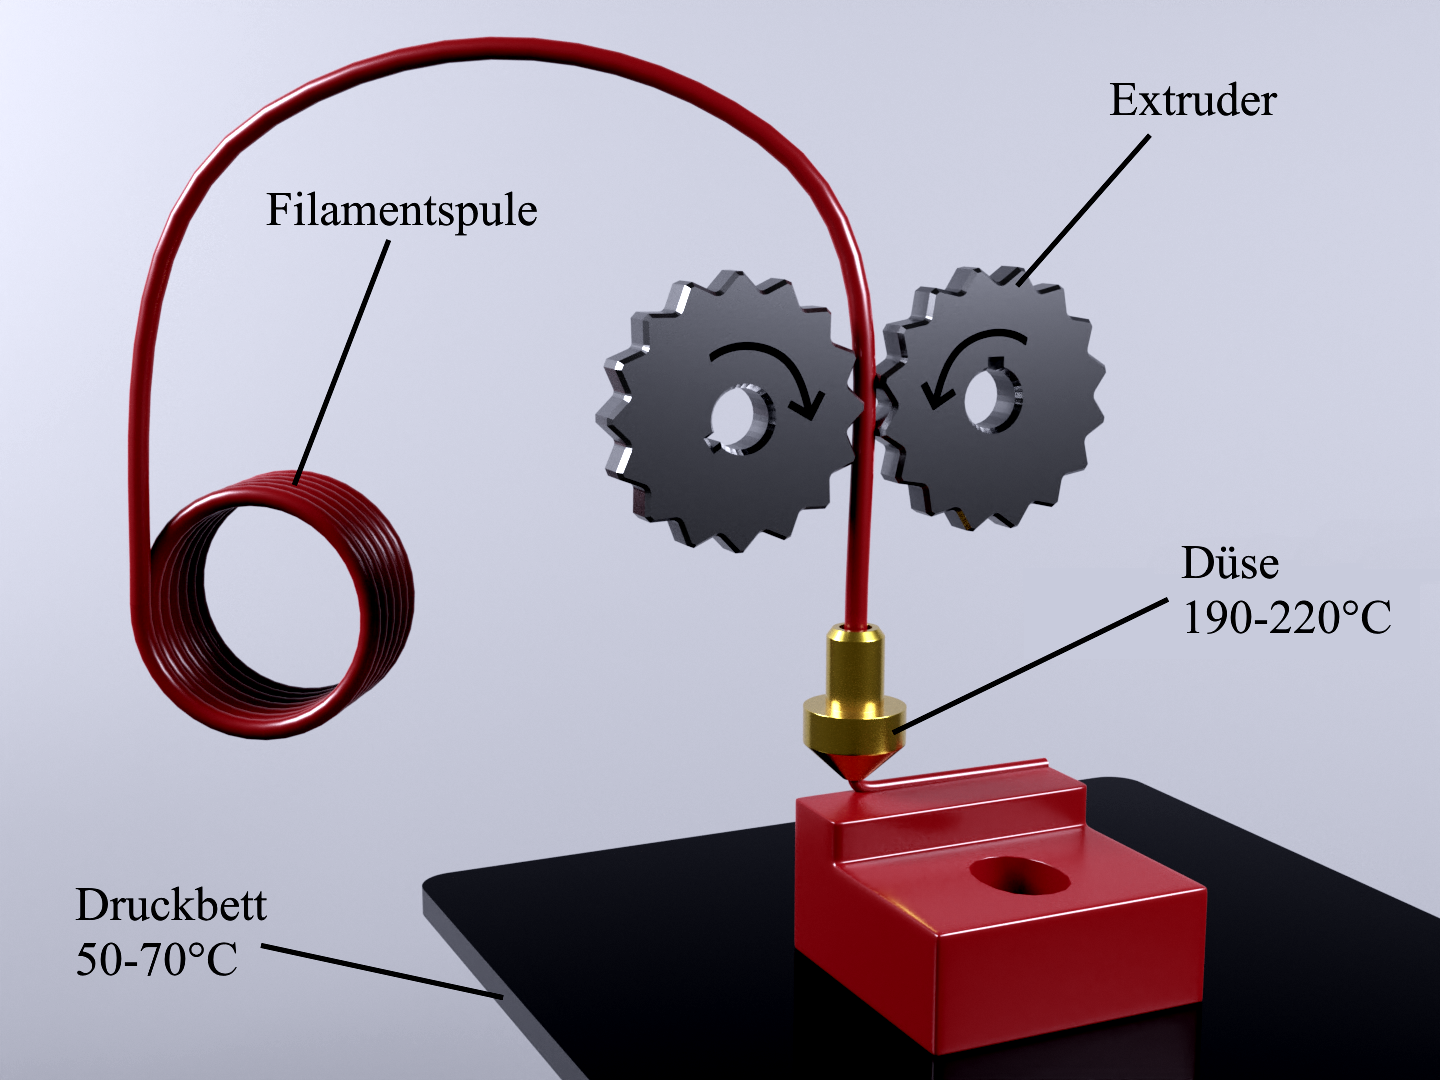
\includegraphics[scale=0.2]{FDM.png}
\caption{FDM-Funktionsweise}
\label{fig:FDM}
\end{figure}

\subsection{DUP-3D-Druck}
\label{subsec:tDUP}
\ac{DUP} ist eines der additiven Fertigungsverfahren, bei dem ein fotosensitives Harz Schicht für Schicht ausgehärtet wird, um ein \ac{3D}-Modell zu fertigen. Bei \ac{DUP} wird eine Plattform kopfüber in einen, mit einem speziellen Harz befüllten, Behälter gesenkt, bis diese eine Schichthöhe vom Boden des Behälters entfernt ist. Der Boden dieses Beckens besteht aus einem durchsichtigen Kunststoff und darunter befindet sich ein \ac{LCD}, welches, anders als herkömmlich, eine \ac{UV}-Leuchtdioden-Matrix als Hintergrundbeleuchtung aufweist. Das \ac{LCD} dient als Schablone und lässt nur dort \ac{UV}-Licht durchscheinen, wo das \ac{UV}-sensitive Harz ausgehärtet (polymerisiert) werden soll . Die erste ausgehärtete Harz-Schicht haftet an der Druckplattform, welche anschließend für die nächste eine Schichthöhe angehoben wird. Somit wird jeweils eine Schicht auf einmal gefertigt (Siehe Abbildung \ref{fig:DUP}).\\ Harz-Drucker sind bekannt dafür, dass sie eine deutlich bessere Druckqualität liefern können, als \ac{FDM}. Der Grund dafür sind zum einen die typischen Schichthöhen von 0.025 bis 0.1 Millimeter sowie die erhöhte Auflösung in x- und y-Richtung, welche abhängig von der \ac{LCD}-Auflösung ist.  Harz-Drucker haben also den großen Vorteil, dass (fast) keine Schicht-Rillen zu erkennen und viel detailliertere Modelle druckbar sind. Die maximale Druckgröße ist in den meisten Fällen kleiner als bei \ac{FDM}-Druckern und liegt im Durchschnitt bei etwa 180*120*200 Millimeter. Die Wellenlänge des \ac{UV}-Lichts der LEDs beträgt zwischen 395 und 405 Nanometer, was ebenfalls dem sensitiven Bereich des Harzes entsprechen muss. Nachdem ein Druck fertiggestellt wurde, ist dieses Modell immer noch mit flüssigem Harz überzogen, welches mit Alkohol entfernt werden muss. Da die Aushärtezeit beim Druckprozess pro Schicht nur circa zwei Sekunden dauert, muss das fertige Modell mit einer \ac{UV}-Lichtquelle erneut für 5 bis 10 Minuten ausgehärtet werden, um seine endgültigen Material-Eigenschaften zu erhalten. Mittlerweile gibt es einige Unternehmen, welche Harze mit besonderen Eigenschaften anbieten, wie zum Beispiel erhöhte Festigkeit, Zähigkeit oder mechanisch bearbeitbar.\\
\ac{DUP} und andere Harz-Druckverfahren haben also den großen Nachteil, dass sehr viel Aufwand im Bezug auf die Nachbearbeitung besteht und immer mit ausreichend Schutzkleidung, wie Handschuhe und Schutzbrille gearbeitet werden muss, da die Harze gesundheitsschädlich sein können. (\cite{druckwegeDUP})
\begin{figure}[h]
\centering
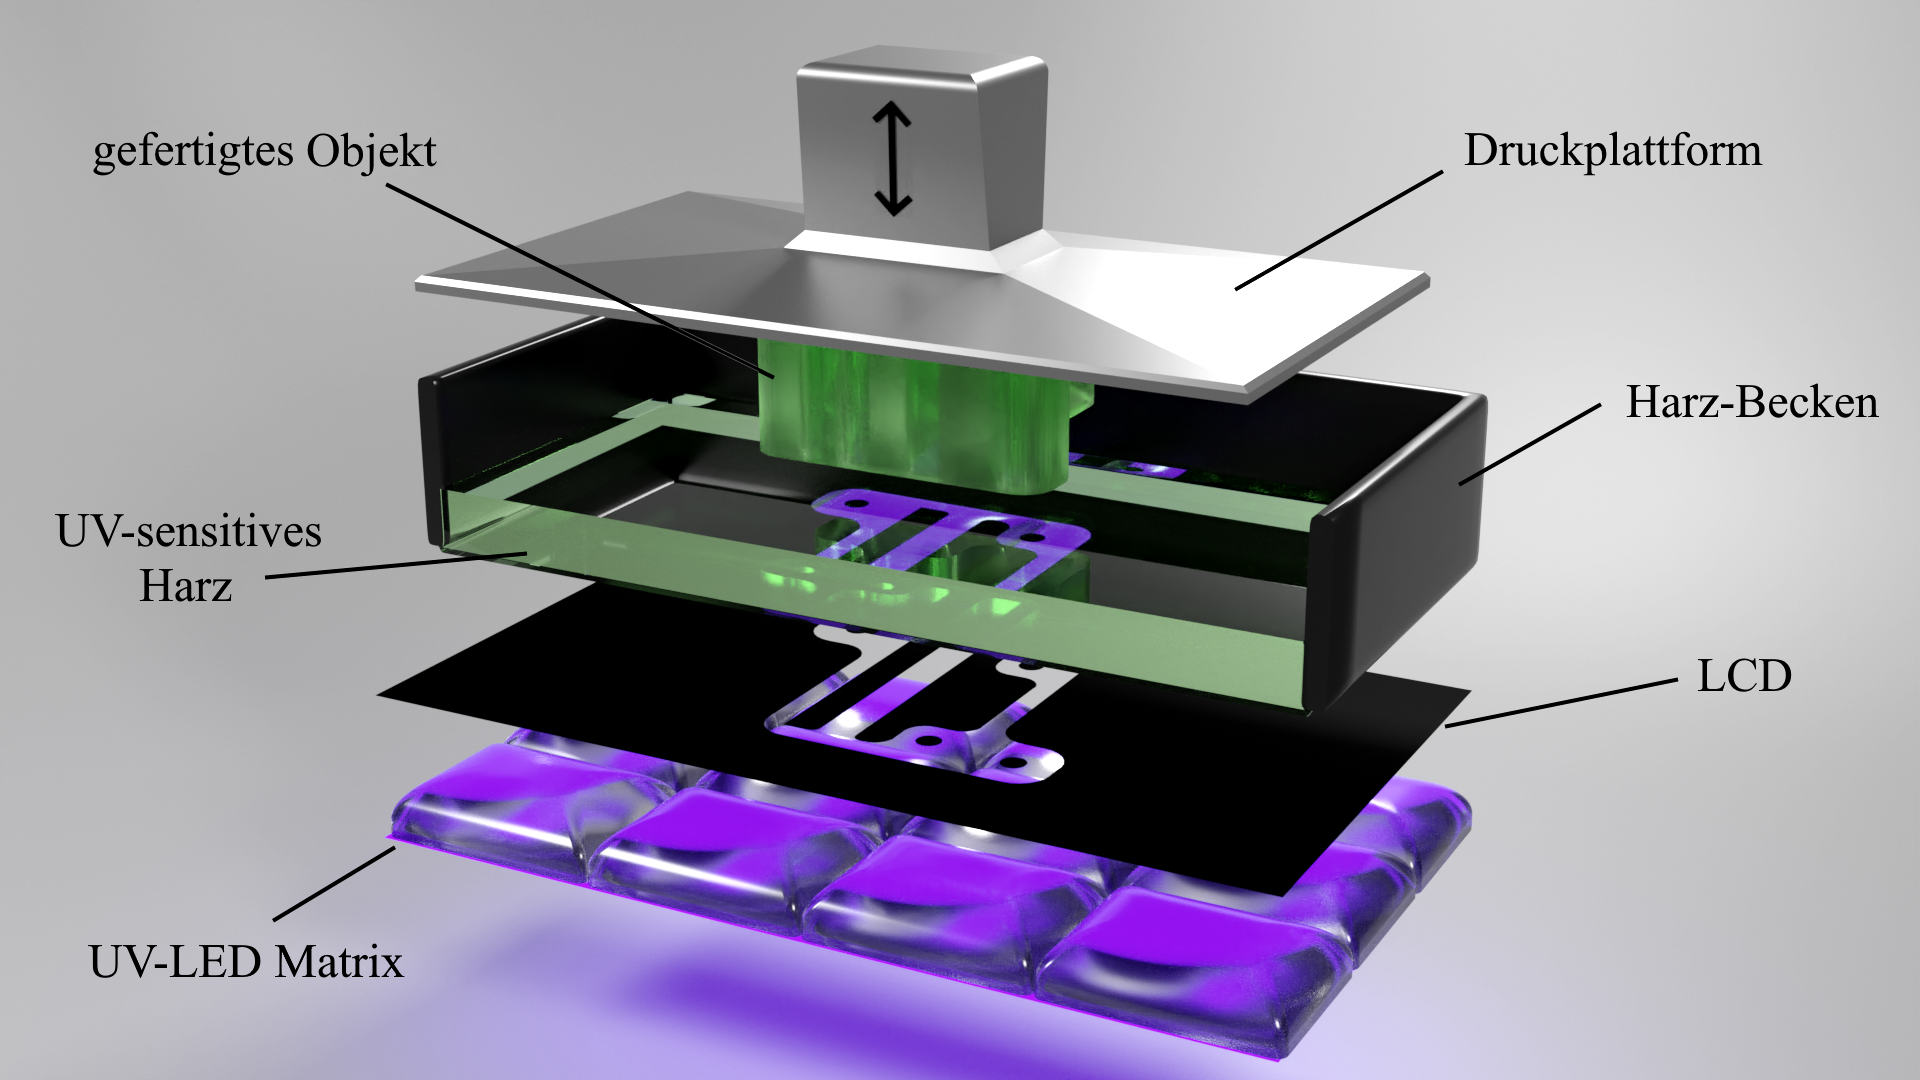
\includegraphics[scale=0.2]{DUP.png}
\caption{DUP-Funktionsweise}
\label{fig:DUP}
\end{figure}
\newpage
\section{Inertiale Messeinheit}
\label{sec:IMU}
\newpage
\section{Drehzahlmessung}
\label{sec:RPM}
Die individuelle Drehzahl aller vier Räder des Modellautos soll erfasst werden. Dafür sind die Auswahl verschiedener Sensortechnologien, die Konstruktion, Fertigung und Montage der Halterungen sowie die Programmierung des Einplatinencomputers notwendig.

\subsection{Wahl der Sensortechnologie}
\label{subsec:RPMchoice}
Aufgrund des Hinterradantriebes des Modellautos sind für die vorderen und hinteren Räder unterschiedliche Sensortypen erforderlich. Durch die Federung des Fahrgestells und der Lenkung der Vorderräder, kommen einige Herausforderungen bei der Sensorwahl und Montage auf. Die Drehzahlerfassung der Hinterräder erfolgt deswegen direkt an den Ausgangswellen des Differentials. Bei den Vorderrädern muss die Drehzahl direkt an den Rädern gemessen werden, da diese nur mitlaufen und keine Antriebswelle aufweisen.\\
Für die Drehzahlmessung der Hinterräder werden Infrarot-Gabellichtschranken, wie in Sektion \ref{subsec:tIR} beschrieben, verwendet. Diese geben die Versorgungsspannung von +3.3 V aus, wenn der \ac{IR}-Strahl unterbrochen wird. Auf der Differentialwelle ist ein Ring mit vier länglich ausgeführten Extrusionen angebracht, welche den Strahl pro Umdrehung der Welle vier mal unterbrechen.

\newpage
\section{Positionsbestimmung}
\label{sec:GPS}
Um die geografische Lage des Autos festzuhalten, wird ein \ac{GPS}-Modul verwendet. Das System \ac{GPS} wird in Sektion \ref{subsec:tGPS} erklärt. Dazu gehört die Wahl der Elektronik, die Montage sowie die programmatische Implementation.

\subsection{Wahl der GPS-Elektronik}
\label{subsec:GPSchoice}
Das GY-NEO6MV2 \ac{GPS}-Modul mit Keramikantenne bietet eine günstige Möglichkeit zur Positionsbestimmung. Mit einer Genauigkeit von 1,5 bis 6 Metern, liefert es die Positionsdaten über die \ac{UART}-Schnittstelle, mithilfe des \ac{NMEA}-Protokolls. Näheres zur Datenübertragung wird in Sektion \ref{subsec:GPSprogram} erklärt. Die Wiederholungsrate der Datenpakete liegt standardmäßig bei 1 \ac{Hz} und kann auf bis zu 5 \ac{Hz} erhöht werden. Die Standard-Baudrate über die serielle Schnittstelle beträgt 9600 $\frac{\mathrm{\ac{b}}}{\mathrm{\ac{s}}}$. Versorgt wird das GY-NEO6MV2 mit 2.7 bis 5 V und arbeitet in einem Temperaturbereich von -40°C bis 85°C. Es hat eine Kaltstart-Zeit von 27 Sekunden und eine Hotstart-Zeit von 1 Sekunde. Ein Kaltstart ist bei einem GPS-Gerät die erste Erfassung von Satellitenbahnen und Zeiten bei der ersten Aktivierung, oder wenn sich das Gerät von der letzten Ortsbestimmung weit entfernt hat. Ein Hotstart tritt bei einer Aktivierung des GPS-Moduls dann auf, wenn es die Satellitendaten noch weiß. Das ist meistens der Fall, wenn nicht mehr als sechs Stunden seit der letzten Positionserfassung vergangen sind und sich das Gerät seit dem nicht weit entfernt hat. Die angegebenen Zeiten sind dabei die kleinstmöglichen. Die dazugehörige Keramikantenne wird über eine UFL-Hirose-Verbindung am GPS-Modul angesteckt. 

\subsection{Montage der GPS-Elektronik}
\label{subsec:GPSmount}
Das GY-NEO6MV2 Modul ist an der Innenseite des Deckels des Elektronikgehäuses mit doppelseitigem Klebeband angebracht. Der Vorteil dieser Montagestelle ist die Fixiermöglichkeit der Antenne. Diese muss, um Satelliten-Daten empfangen zu können, in den freien Himmel zeigen. Über eine Bohrung im Deckel des Gehäuses der Elektronik ist die Antenne mit der Platine verbunden.
\newpage
\begin{figure}[h]
\centering
\includegraphics[scale=0.2]{GPSMount.png}
\caption{Montage des \ac{GPS}-Moduls}
\label{fig:GPSMount}
\end{figure}

\subsection{Programmatische Implementation}
\label{subsec:GPSprogram}
Wie bereits erwähnt liefert das GPS-Modul die Daten über die UART-Schnittstelle. Dabei wird die transmit (TX)-Leitung des GPS-Moduls mit dem receive (RX)-Pin des Raspberry Pi verbunden. Die receive-Leitung des Moduls ist nicht nötig, da es nur die Daten an den \ac{Raspi} senden soll.\\
Um den seriellen (\ac{UART}) Port des Raspberry Pi verwenden zu können muss dieser zunächst in der Konfigurationsdatei  \verb|/boot/config.txt| mit dem Hinzufügen der Zeile \verb|enable_uart=1| aktiviert werden. Des Weiteren muss die Konsole \glqq getty\grqq\ der seriellen Schnittstelle \verb|/dev/ttyAMA0| deaktiviert werden, um diese in einem Python Programm einbinden zu können. Dazu ist einerseits der Befehl \verb|sudo systemctl stop serial-getty@ttyAMA0.service|\ notwendig, um den Prozess zu stoppen, andererseits muss der Befehlt \verb|sudo systemctl disable serial-getty@ttyAMA0.service| verwendet werden, um das automatische Initialisieren des Prozesses durch systemd zu unterbinden.\\
Das \ac{GPS}-Modul gibt die Daten mit dem \ac{NMEA}-Protokoll, welches der Standard in der GPS-Technik ist, an den Raspberry Pi weiter. Der Inhalt eines Datenpaketes in diesem Format sieht wie in Abbildung \ref{fig:NMEA} dargestellt aus. Wie zu erkennen ist, bestehen diese \ac{GPS}-Daten aus mehreren \ac{GPS}-Nachrichten. Jede dieser verschiedenen Nachrichten (Zeilen) wird durch einen sogenannten Protokoll-Header gekennzeichnet. Diese sind GPGGA, GPGSA, GPGSV, GPGLL, GPRMC und GPVTG. Nachfolgend an den Header stehen die verschiedenen Informationen mit Komma getrennt. Dieses Format hat sich gerade deswegen durchgesetzt, da es eine Vielzahl an Informationen beinhaltet und es dem Programmierer überlassen ist, welche Informationen er davon verwenden möchte. Bei den unterschiedlichen Headern sind die Daten verschieden, beziehungsweise in einer anderen Reihenfolge angeordnet. Der Header GPRMC wird hier verwendet, da er die Längen- und Breitengrade klar erkenntlich und einfach beinhaltet. Die Inhalte und Reihenfolge der Daten ist folgendermaßen aufgebaut: An erster Stelle befindet sich die koordinierte Weltzeit (UTC) in jeweils zweistelligen Stunden, Minuten und Sekunden. Danach folgt der Status. Ein A steht für \glqq data valid\grqq , ein V für \glqq data not valid\grqq . An der nächsten Stelle steht der Breitengrad (latitude), danach folgt die Kennzeichnung mit einem N oder S für \glqq nördliche oder südliche Breite\grqq . Der Längengrad (longitude) steht als nächstes, mit der Kennzeichnung W oder E für \glqq westliche oder östliche Länge\grqq . Die Einheit der Längen- und Breitengrade ist dabei Grad und anschließend Minuten als Dezimalzahl. Die Positionsdaten 4728.545 N, 01524.038 E entsprechen beispielsweise den Koordinaten 47° 28.545' N und 15° 24.038' E.

\begin{figure}[h]
\centering
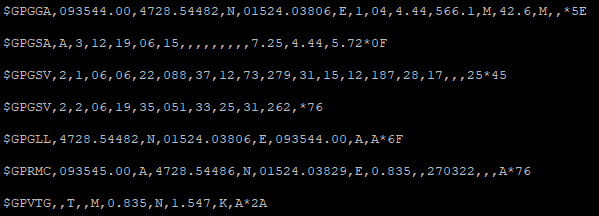
\includegraphics[scale=0.8]{NMEA.png}
\caption{Daten des GPS-Moduls im NMEA-Format}
\label{fig:NMEA}
\end{figure}

Um diese Positionsdaten programmatisch herauszufiltern, wird jede GPS-Nachricht auf ihre ersten sechs Zeichen überprüft. sollten diese \verb|$GPRMC| entsprechen, wird mithilfe der pynmea2 Bibliothek, wie in Sektion \ref{subsubsec:tpynmea2} beschrieben, die Daten der Breiten- und Längengrade auf zwei Variablen geschrieben. Diese Positionsdaten werden automatisch in Grad als Dezimalzahl formatiert. 
\newpage
\section{Elektronischer Aufbau}
\label{sec:Elektronik}
Um ein gesamtes funktionsfähiges Mess- und Verarbeitungssystem realisieren zu können, sind mehrere Schritte, hinsichtlich des mechanischen und elektronischen Aufbaus notwendig. Dazu zählen unter anderem die Wahl der Hardwareplattform, die Auslegung eines Spannungsversorgungssystems und Möglichkeiten, den Zustand des Programmes erkennen und ändern zu können. Außerdem ist ein robustes Gehäuse zur Einhausung dieser Komponenten sowie mehrerer Sensoren zu konstruieren und fertigen. Zusätzlich sind externe, im Gehäuse nicht verbaute Sensoren, über eine zuverlässige Verbindung in das Elektroniksystem einzubinden.

\subsection{Wahl der Hardware-Plattform}
\label{subsec:elekMikrocontroller}
An die Hardware-Plattform werden einige Anforderungen gestellt. Sie muss Möglichkeiten zur Kommunikation mit den Sensoren bieten, außerdem muss sie genug Rechenleistung aufbringen können, um alle Sensoren simultan auszulesen und diese Daten für die spätere Verwendung aufzuzeichnen. Es sollten außerdem Optionen vorhanden sein, die gesammelten Daten vom ferngesteuerten Auto zu exportieren, um sie auf einem anderen Gerät auszuwerten. Eine weitere essentielle Eigenschaft ist, in welchen Programmiersprachen die Hardware programmiert werden kann, da die Verfügbarkeit von Bibliotheken für die jeweilige Programmiersprache eine wichtige Rolle spielt. Andere Faktoren, die zwar nicht notwendig sind, aber von großem Nutzen sein können, sind \ac{WLAN}- und Bluetooth-Funktionalität. Die bekanntesten Hersteller von solchen Plattformen sind Raspberry Pi und Arduino.  Beide Hersteller bieten sowohl größere und leistungsstärkere als auch kleinere, leistungsschwächere Optionen an. Die bekanntesten Optionen sind somit der Raspberry Pi 4 Model B, der Raspberry Pi Zero 2 W, der Arduino Uno und der Arduino Nano.
\begin{table}[h]
\centering
\begin{tabular}{|c||c|c|c|c|} 
\hline
Plattform                                                      & Arduino Uno                                                                                 & Arduino Nano                                                                                & Raspi 4B                                                                                           & Raspi Zero 2 W                                                                             \\ 
\hhline{|=::====|}
Prozessor                                                      & ATmega328P                                                                                  & ATmega328                                                                                   & BCM2711                                                                                            & Cortex-A53                                                                                \\ 
\hline
Schnittstellen                                                 & \begin{tabular}[c]{@{}c@{}}UART\\SPI\\I$^2$C\\6 analoge Pins\\14 digitale Pins\end{tabular} & \begin{tabular}[c]{@{}c@{}}UART\\SPI\\I$^2$C\\8 analoge Pins\\12 digitale Pins\end{tabular} & \begin{tabular}[c]{@{}c@{}}UART\\SPI\\I$^2$C\\28 GPIO Pins \\4 USB Ports\\RJ45 Buchse\end{tabular} & \begin{tabular}[c]{@{}c@{}}UART\\SPI\\I$^2$C\\28 GPIO Pins \\micro USB Port\end{tabular}  \\ 
\hline
\begin{tabular}[c]{@{}c@{}}Programmier-\\sprachen\end{tabular} & C, C++                                                                                      & C, C++                                                                                      & \begin{tabular}[c]{@{}c@{}}Python\\C, C++\\Scratch\end{tabular}                                    & \begin{tabular}[c]{@{}c@{}}Python\\C, C++\\Scratch\end{tabular}                           \\ 
\hline
\begin{tabular}[c]{@{}c@{}}Zusatz-\\funktionen\end{tabular}    & -                                                                                           & -                                                                                           & WLAN, Bluetooth                                                                                    & WLAN, Bluetooth                                                                           \\ 
\hline
Preis                                                          & 20\officialeuro                                                                                                                                                                                   & 18\officialeuro                                                                                          & ab \$35                                                                                            & \$15                                                                                      \\
\hline
\end{tabular}
\caption{Vergleich von verschiedenen Hardware-Plattformen}
\label{tab:myCcomparison}
\end{table}
\\
Da auf dem Raspberry Pi wie in Sektion \ref{subsec:tRasPiOS} beschrieben eine vollwertige Linux-Distribution läuft, können auf Einplatinencomputer von Raspberry Pi alle programmiersprachen verwendet werden, die unter Linux unterstützt sind. Die in der Tabelle aufgelisteten Sprachen sind die, die von Raspberry Pi OS standardmäßig unterstützt werden, ohne eigens Pakete installieren zu müssen.\\
Aufgrund der im Vergleich zum ATmega328 hohen Rechenleistung des Arm Cortex-A53, der Option, Einplatinencomputer von Raspberry Pi mit Python zu programmieren, der zusätzlichen \ac{WLAN}-Funktion und den niedrigen Preises wird der Raspberry Pi Zero 2 W verwendet. Ein weiterer Vorteil des Raspberry Pi ist es, dass er einen eingebauten microSD Kartenslot hat, die damit verwendete microSD Karte dient als Hauptspeicher des Einplatinencomputers. Dieses Speichermedium kann deswegen auch gleich für das Aufzeichnen der Daten verwendet werden, somit entfällt die Notwendigkeit für ein externes SD-Kartenmodul, welches bei einem Arduino notwendig wäre.

\subsection{Spannungsversorgung}
\label{subsec:elekSupply}
Da das Auto, wie in Sektion \ref{sec:Auto} beschrieben, mit zwei 7.4\ac{V} Lithium Polymer Akkus betrieben wird, bietet sich die Möglichkeit an, diese auch für die Versorgung der Messelektronik zu verwenden. Um die Akkus gleichmäßig zu belasten werden beide in Serie geschalteten Akkus für diese Spannungsversorgung verwendet. Damit stehen 14.8\ac{V} zur Verfügung, welche mit einem DC-DC Stepdown-Converter auf 5\ac{V}, was der Versorgungsspannung des Raspberry Pi entspricht, herabgewandelt werden. Der DC-DC-Converter weist am Eingang zwei Schraubklemmen sowie eine Hohlbuchse auf. Die Leitungen der Akkus werden an den Schraubklemmen am Eingang des Converters angeschlossen. Ein Kippschalter, der die Plus-Leitung unterbrechen kann, ermöglicht das manuelle Aus- und Einschalten der gesamten Messelektronik. Zusätzlich wird ein Voltmeter mit Siebensegmentanzeige an der Hohlsteckerverbindung am Eingang angeschlossen, welches die Akkuspannung anzeigt (Siehe Abbildung \ref{fig:switch}). Der Stepdown-Wandler weist am Ausgang ebenfalls zwei Schraubklemmen und zusätzlich eine \ac{USB}-A-Buchse auf. Da der Raspberry Pi als Versorgungsanschluss eine Micro-\ac{USB}-Buchse verbaut hat, wird ein USB-A zu Micro-\ac{USB} Kabel gekürzt und als Versorgungsleitung verwendet. Die Spannungsversorgung der einzelnen Sensoren erfolgt über die 3.3\ac{V}, 5\ac{V} und GND Pins des Raspberry Pi. 

\begin{figure}[h]
\centering
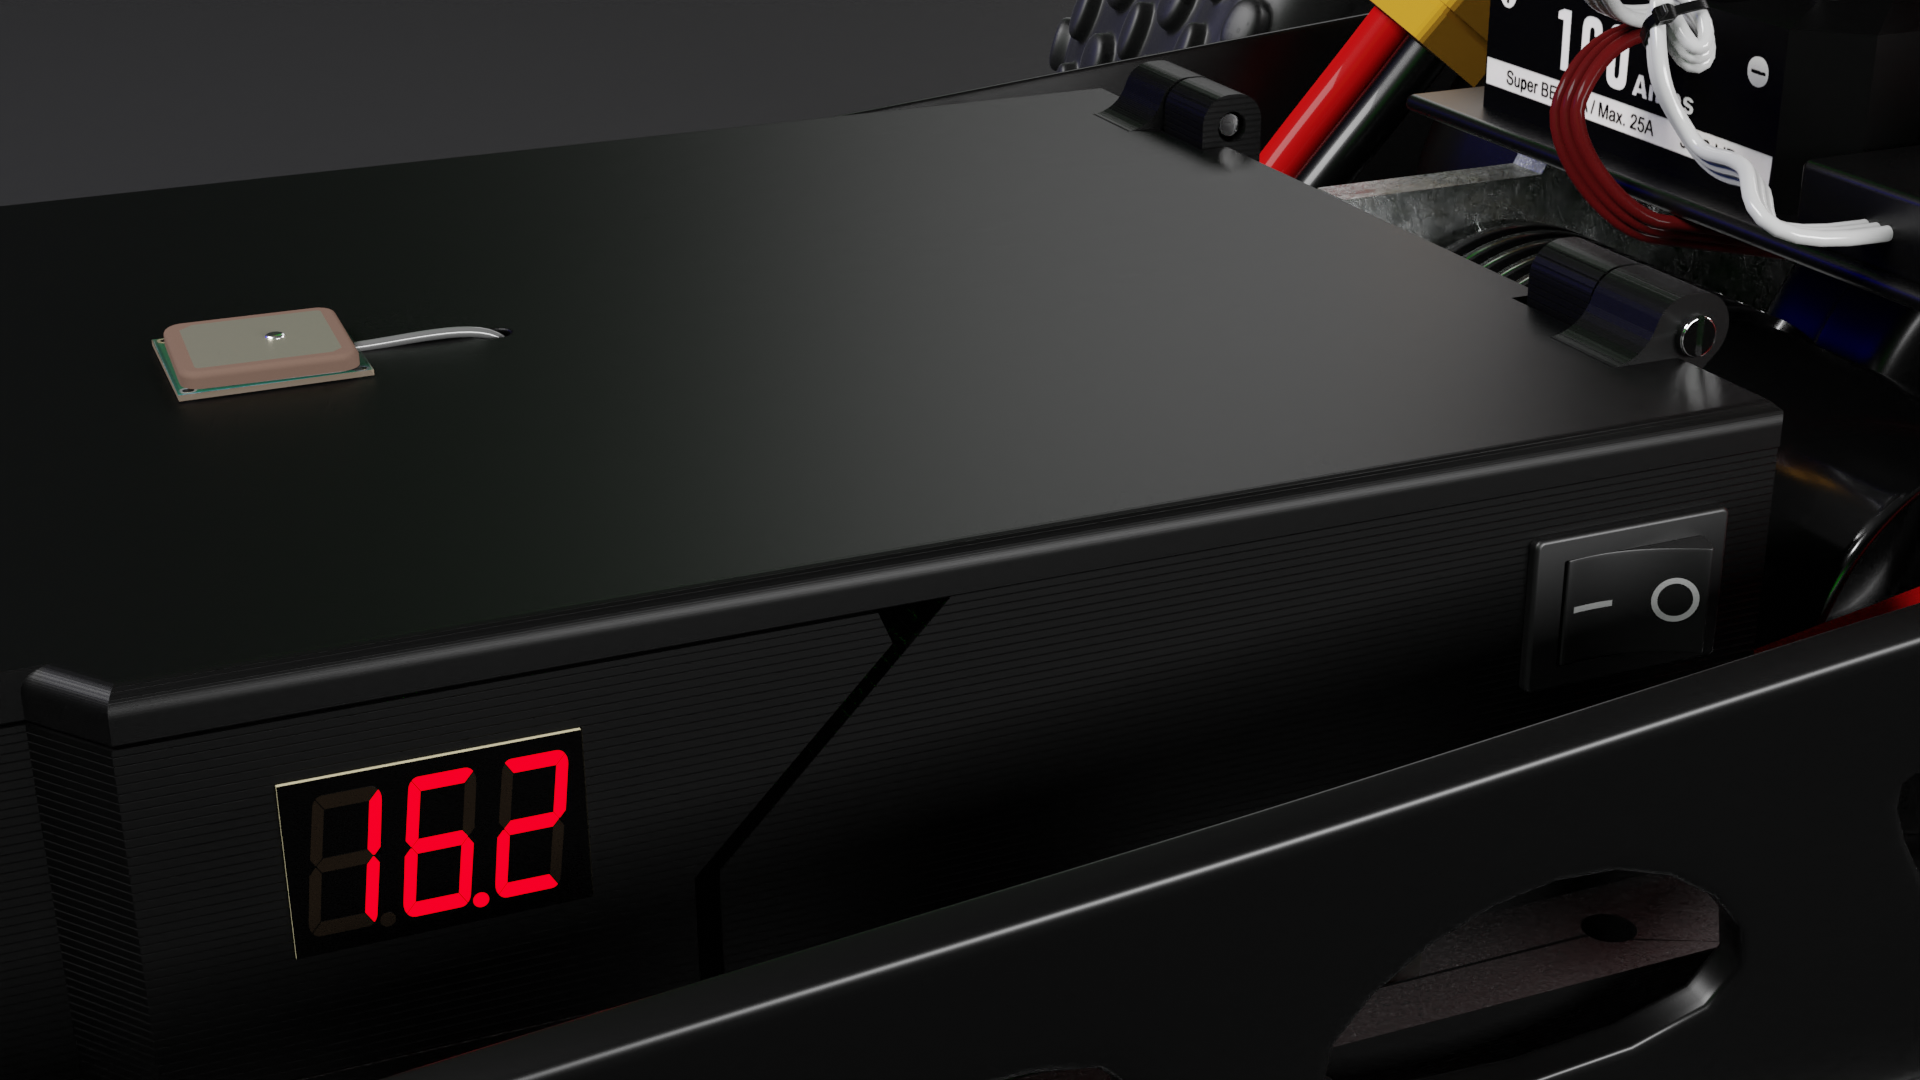
\includegraphics[scale=0.2]{switch.png}
\caption{7-Segmentanzeige und Kippschalter im Gehäuse}
\label{fig:switch}
\end{figure}

\subsection{Gehäuse}
\label{subsec:elekCasing}
Eine robuste, vielseitige Einhausung der Messelektronik ist essentiell, um diese stabil montieren sowie von äußeren Einflüssen wie Staub und Sand schützen zu können. Die Sitzkonstruktion des Autos wird entfernt, wodurch Raum für ein Gehäuse freigelegt wird. Als Basis dient eine einfache Plattform, welche an den ursprünglichen Montagestellen der Sitzkonstruktion in das Auto geschraubt wird. Direkt darunter, auf der Bodenplatte des Autos, befinden sich die Akkus. Auf diese Plattform werden mehrere Seitenwände aufgeschraubt.\\
Sämtliche Schraubverbindungen im und am Gehäuse werden mittels M3 Gewindeeinsätzen ermöglicht. Die \ac{FDM}-3D-gedruckten Gehäusekomponenten weisen Bohrungen auf, in welche diese Gewindeeinsätze eingeschmolzen werden. Diese Lösung, Schraubverbindungen in 3D-Druck-Komponenten zu ermöglichen, ist sehr belastbar und einfach umzusetzen, weshalb sie häufig eingesetzt wird. \\
Die U-förmige Rück- und gleichzeitig hintere Seitenwand, weist in Bodennähe eine rechteckige Ausnehmung auf, welche für die Durchführung der Versorgungsleitungen sowie den Sensorleitungen der hinteren Drehzahlsensoren vorgesehen ist. Auf der rechten Seite dieser Wand ist der Kippschalter der Versorgungsleitung eingefasst. Links befindet sich die \ac{USB}-A-Buchse für die Datenübertragung mittels \ac{USB}-Datenträger, wie es in Sektion \ref{subsec:Datenübertragungsmodus} näher beschrieben wird.
\begin{figure}[h]
\centering
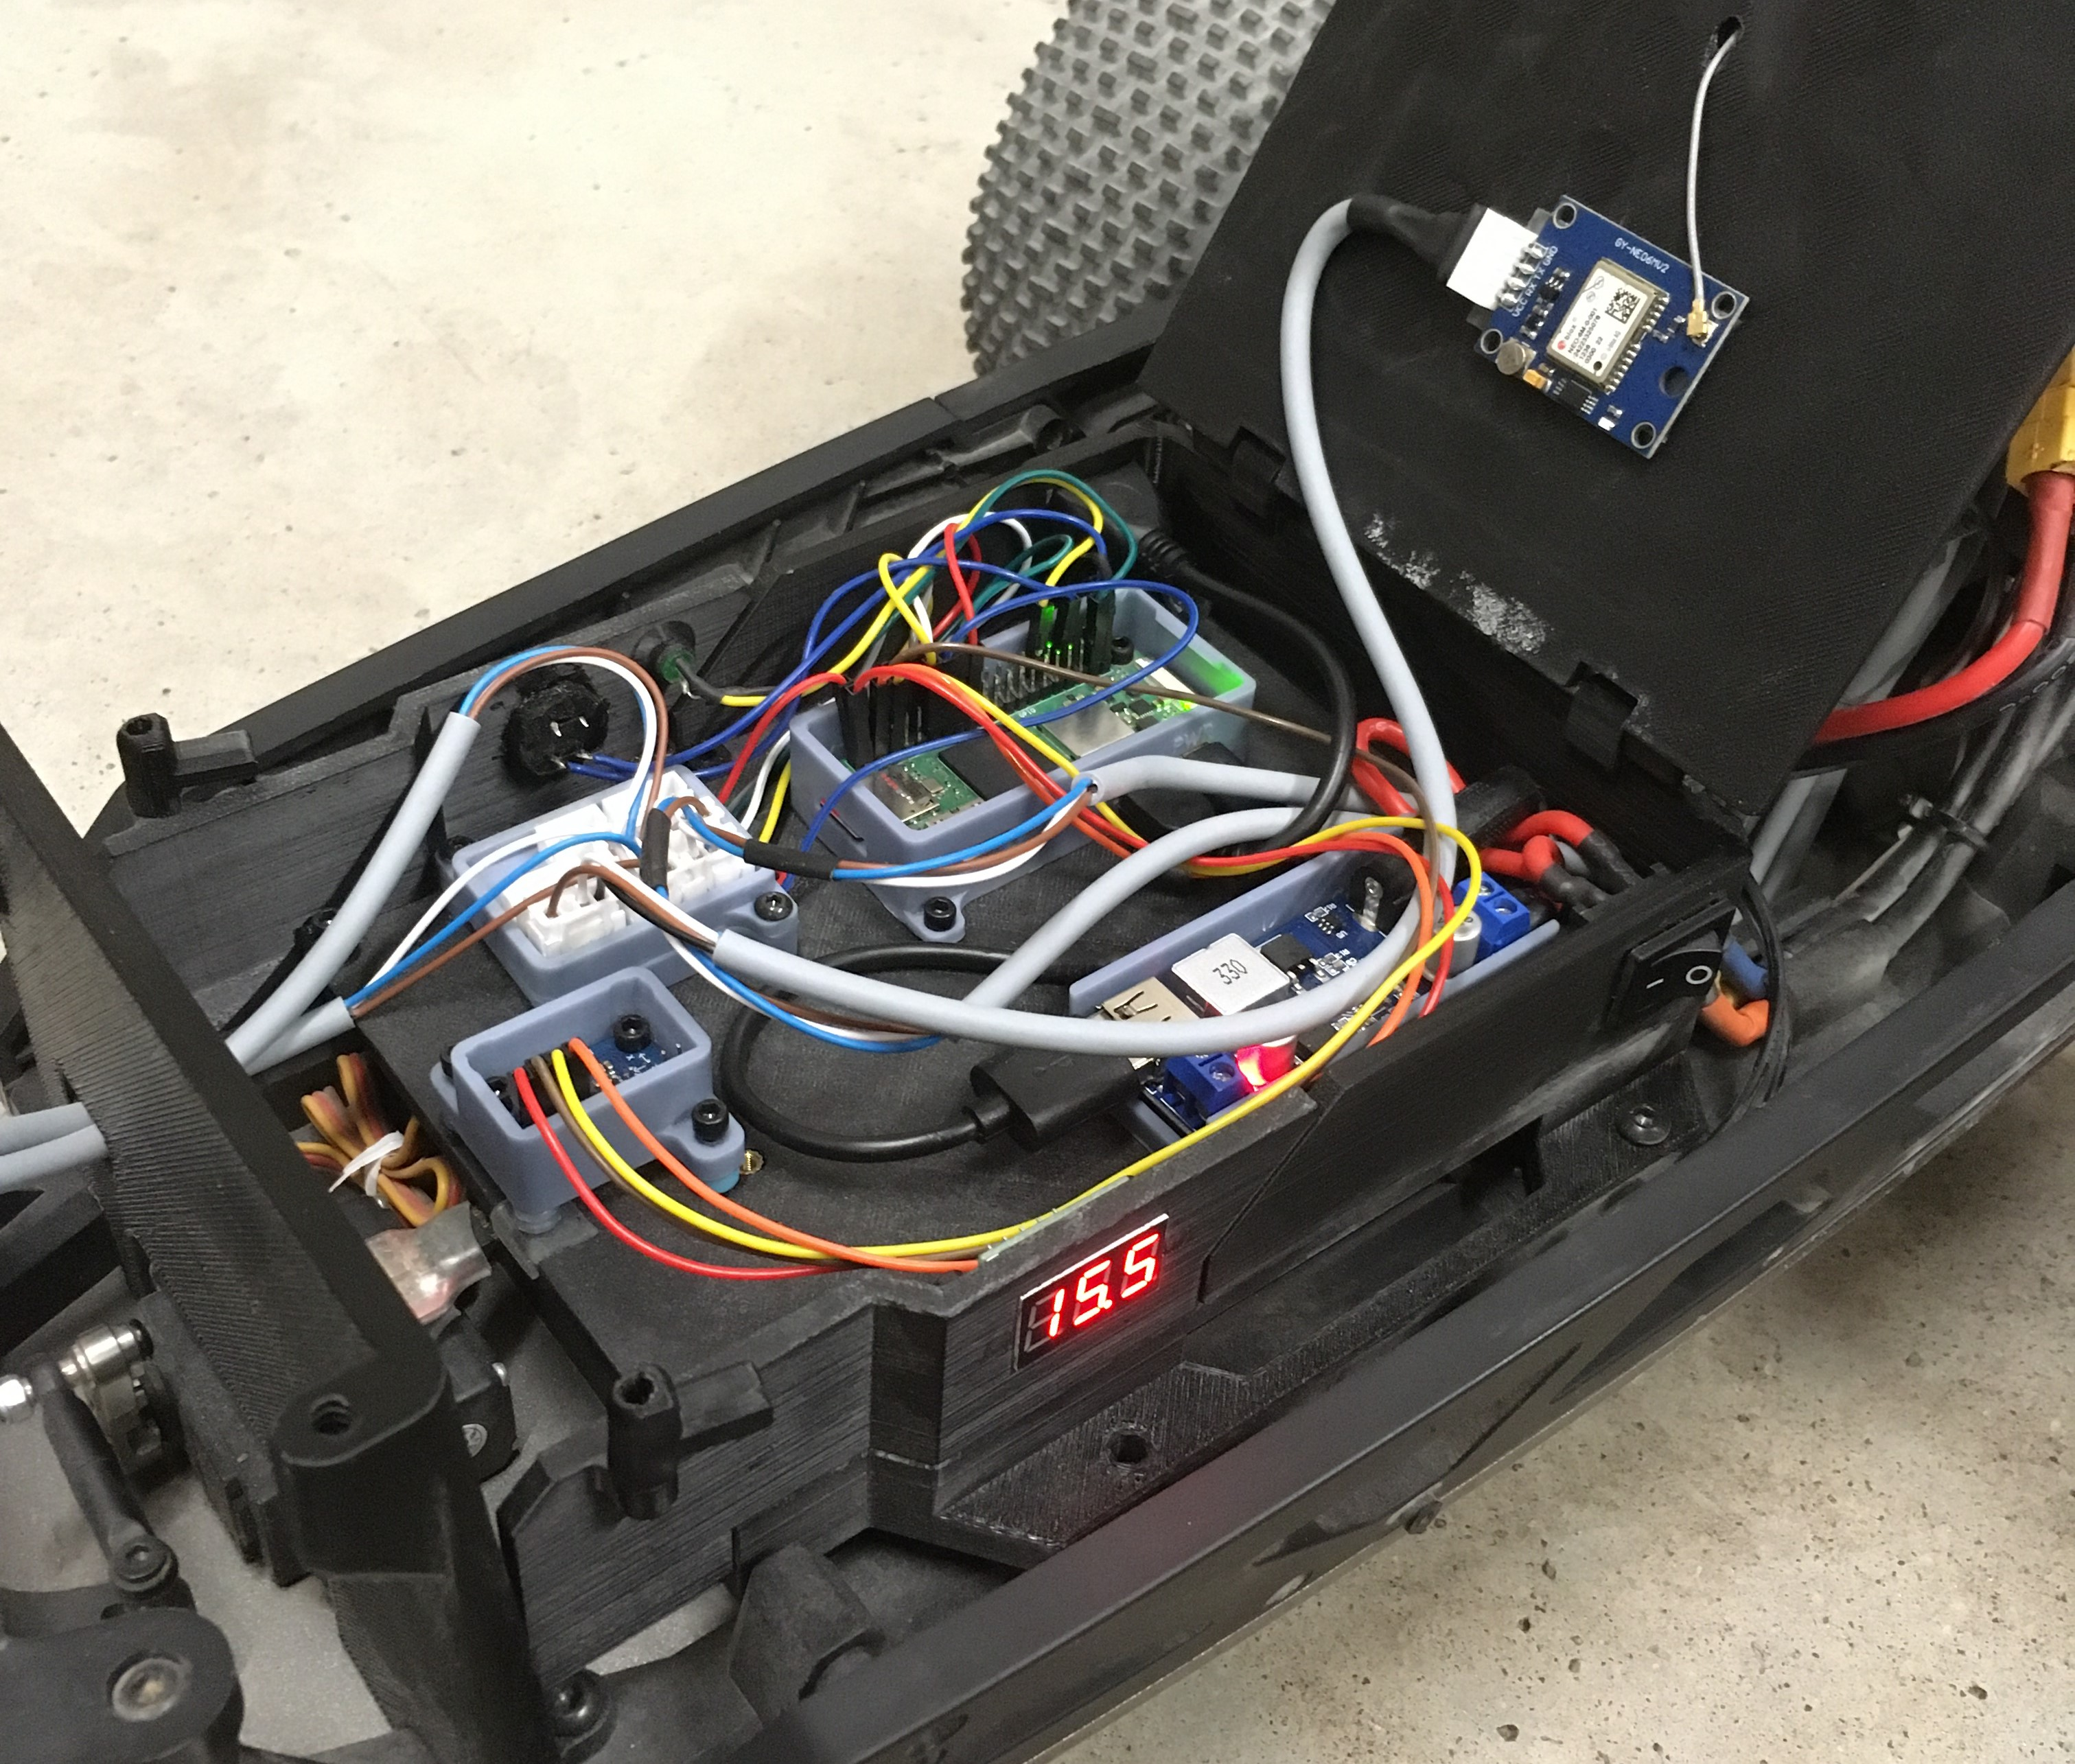
\includegraphics[scale=0.1]{Electronics.jpg}
\caption{Elektronik im Gehäuse}
\label{fig:elekCase}
\end{figure}
\\
An der hinteren Oberkante dieser Komponente sind außerdem zwei Scharniere ausgeführt, um den Deckel einfach öffnen und schließen zu können. Am vorderen Ende der Plattform ist links und rechts jeweils eine weitere Wandkonstruktion angebracht, welche mit der hinteren mit einem schmalen Abstand abschließt. Auf der rechten Wand befindet sich ein Taster für das Umschalten des Programmzustandes sowie eine \ac{RGB}-\ac{LED}, die diesen Zustand signalisiert. In der linken vorderen Wand ist die Siebensegmentanzeige eingebaut, welche die aktuelle Akkuspannung anzeigt. Diese vorderen Wandteile weisen außerdem eine Montagemöglichkeit für die Deckelverriegelungen auf. Der Deckel des Gehäuses deckt den gesamten Innenraum ab und kann durch die bereits erwähnten Scharniere auf- und zugeklappt werden. Mit Hilfe von zwei Drehverriegelungen wird der Deckel geschlossen gehalten. Wie in Sektion \ref{subsec:GPSmount} beschrieben, befindet sich im Deckel eine Bohrung für die Durchführung der GPS-Antennenleitung.\\
Um den Raspberry Pi und beispielsweise den Stepdown-Wandler auf der Grundplattform zu montieren, weist diese ebenfalls Bohrungen mit eingeschmolzenen Gewindeeinsätzen auf. Für die Montage sind außerdem einzelne Gehäuse für den Raspberry Pi und Stepdown-Wandler notwendig. Diese wurden mittels \ac{CAD} konstruiert und anschließend mit dem in Sektion \ref{subsec:tDUP} beschriebenen \ac{DUP}-Verfahren 3D-gedruckt. Da der Raspberry Pi Bohrungen in den Ecken aufweist, wird dieser mit M3 Schrauben in seinem Gehäuse montiert. Der Stepdown-Wandler hat keine Befestigungsbohrungen und wird deshalb mit doppelseitigem Klebeband befestigt. 
\begin{figure}[h]
\centering
\includegraphics[scale=0.2]{Elektronik_Raspi.png}
\caption{JST-Anschlusseinheit und Raspberry Pi}
\label{fig:JST_Raspi}
\end{figure}

\subsection{Einbindung externer Elektronik}
\label{subsec:elekExtern}
Wie in Sektion \ref{subsec:RPMmount} bereits erklärt, sind die Drehzahlsensoren in der Nähe aller vier Räder angebracht. Eine zuverlässige Verbindung dieser Sensoren mit dem Raspberry Pi ist ausschlaggebend. Besonders bei den Vorderrädern, welche durch die Federung sowie die Lenkung Bewegungen ausführen ist eine robuste, aber flexible Verbindung zum Gehäuse notwendig. Aus diesem Grund werden als Verbindungselemente JST-XH Stecker und Buchsen verwendet und eine biegsame Mantelleitung zur Versorgung und Signalübertragung. Eine Mantelleitung hat den Vorteil, dass sie mehrere Adern mit einem Mantel umschließt, der es ermöglicht die Leitung stabil am Fahrgestell zu fixieren und die einzelnen Adern gegen mechanische Beanspruchung schützt. Auf diese Weise können die Sensoren außerdem an- und abgeschlossen werden.\\
Die insgesamt vier Mantelleitungen werden durch dementsprechende Ausnehmungen an den Gehäusewänden in das Innere des Gehäuses geführt. Um das Anschließen der Drehzahlsensoren zu vereinfachen, werden diese auf einer Anschlusskonstruktion mit mehreren JST-XH Buchsen angesteckt. Diese Buchsen sind bereits mit den korrekten Pins am Raspberry Pi verbunden. Auch das \ac{GPS}-Modul ist mit einer solchen Mantelleitung und JST-XH Verbindungen an dieser Anschlusseinheit angeschlossen.\\
Um den in Sektion \ref{subsec:Datenübertragungsmodus} beschriebenen Datenübertragungsmodus nutzen zu können, ist eine \ac{USB}-A-Buchse, welche von außerhalb des Gehäuses zugänglich sein muss, zu installieren. Diese von Außen zugängliche Buchse wird mithilfe eines micro-\ac{USB} auf \ac{USB}-A-Adapters, welcher an der Datenbuchse des Raspberry Pi angeschlossen ist, realisiert.
\newpage
\section{Datenverarbeitung}
\label{sec:Datenverarbeitung}
Der \ac{Raspi} ist für die Datenverarbeitung zuständig, einerseits empfängt er die Daten von den verschiedenen Sensoren, andererseits schreibt er alle gesammelten Messwerte auf die microSD-Karte. Diese Operationen werden alle von einem Python-Programm erledigt. Mithilfe eines Tasters kann zwischen zwei Modi umgeschalten werden, einer davon ist der Datenaufzeichnungsmodus, welcher durch eine eingeschaltete \ac{LED} indiziert wird. In diesem Modus werden die Daten von allen verbauten Sensoren gesammelt und anschließend auf den Speicher des \ac{Raspi} geschrieben. Jedes mal, wenn das Programm gestartet wird, wird eine neue Textdatei mithilfe der in Python integrierten Funktion \verb|open()| erstellt. Das von dieser Funktion zurückgegebene Objekt wird dann verwendet, um die erstellte Datei zu bearbeiten. Wenn ein neuer Datensatz gesammelt wird, wird dieser in eine neue Zeile in die Datei geschrieben. Jeder Datensatz besteht aus der Zeit der Datenaufnahme, der Orientierung, den Beschleunigungen, der Umgebungstemperatur, den Drehzahlen, der Geschwindigkeit und den Koordinaten. Die jeweiligen Werte sind voneinander mit Kommas getrennt, um die Kompatibilität mit Tabellenkalkulationsprogrammen wie Microsoft Excel oder LibreOffice Calc zu gewährleisten. Der andere zur Verfügung stehende Modus ist der der Datenübertragung auf ein \ac{USB}-Wechselmedium. In diesem Modus überprüft der Raspberry Pi jede Sekunde, ob an dem Einhängepunkt \verb|/media/usb0| ein Gerät erscheint. Sollte dies geschehen, werden alle erstellten Dateien in 100 Millisekunden-Abständen das Stammverzeichnis des \ac{USB}-Wechselmediums kopiert. Um einen erfolgreichen Kopiervorgang zu signalisieren, blinkt die eingebaute \ac{LED} pro kopierter Datei einmal. Dafür sollte der Datenträger mit einem Dateisystem wie \ac{NTFS} oder \ac{FAT} formatiert sein, welches sowohl unter Linux als auch unter Microsoft Windows eingehängt werden kann. 
\\
Zusätzlich zur Speicherung auf dem Raspberry Pi werden die Daten live in die Befehlszeile ausgegeben, in der das Programm ausgeführt wird. Somit können die Daten live auf einem Computer oder Smartphone ausgelesen werden, solange sich das Auto in Reichweite eines \ac{WLAN} Signals befindet und sich die Geräte im selben Netzwerk befinden. Um diese live-Übertragung zu verwenden, kann das Gerät, auf dem die Daten angezeigt werden sollen via \ac{SSH} mit dem Raspberry Pi verbunden werden und dann das Programm ausführen.
\newpage
\section{Visualisierung}
\label{sec:DesktopApp}
Diese Sektion beschreibt die Bedienung und Funktionsweise der eigens entwickelten Desktopanwendung, welche zur einfachen Visualisierung und Auswertung der Daten dient.
\subsection{Grundlagen}
\label{subsec:VisGrundlagen}
Für die Programmierung der Desktopanwendung wird ebenfalls Python verwendet, in diesem Fall wird zusätzlich auch Qt verwendet. Qt ist, wie in Sektion \ref{subsubsec:tQt} beschreiben, eine Bibliothek zur Entwicklung von grafischen Oberflächen, was eine Erleichterung in der Entwicklung von Desktopanwendungen darstellt. Die Desktopanwendung dieser Diplomarbeit ist in vier Ansichten aufgeteilt. Wird das Programm gestartet, wird zunächst die \glqq Overview\grqq\ angezeigt. In dieser Ansicht sind ein \ac{3D}-Modell des Autos und drei Schaltflächen zu sehen. Die Schaltflächen führen zu den anderen Ansichten, darunter die \glqq Table View\grqq , die \glqq Plot View\grqq \ und die \glqq Map View\grqq . Die Anwendung verfügt außerdem über eine Werkzeugleiste am oberen Rand des Fensters, welche die Funktionen \glqq Schließen\grqq\ und \glqq Vollbild\grqq\ sowie Verknüpfungen zu den Ansichten \glqq Overview\grqq , \glqq Table View\grqq , \glqq Plot View\grqq\  und \glqq Map View\grqq\ enthält.
\begin{figure}[h]
\centering
\missingfigure{}
\caption{Übersichtsseite der Desktopanwendung}
\label{fig:Overview}
\end{figure}
\\
\subsection{Table View}
\label{subsec:VisTableView}
Eine weitere Ansicht ist, wie bereits erwähnt, die \glqq Table View\grqq , in welcher eine Tabelle mit allen Messwerten der geöffneten Datei zu sehen ist. In der Table View sind wie in Abbildung \ref{fig:TableView} abgebildet am oberen Rand der Tabelle Identifikatoren zu sehen, welche die Aufgabe haben, die Werte realen Größen zuordenbar zu machen.
\begin{figure}[h]
\centering
\missingfigure{}
\caption{Table View}
\label{fig:TableView}
\end{figure}
\\
Die Tabelle wird mithilfe des Qt-Widgets \glqq QTableWidget\grqq\ erstellt und angezeigt. Dazu werden die Zeiten als Beschriftungen der Zeilen und die Namen der Messwerte als Beschriftung der Spalten verwendet. 

\subsection{Plot View}
\label{subsec:VisPlotView}
Da eine Tabelle unübersichtlich sein kann und Menschen reine Zahlenwerte oft nicht mit Fahrverhältnissen in Verbindung bringen können, gibt es auch die \glqq Plot View\grqq . In dieser Ansicht werden alle Werte in einem Graphen gezeichnet.
\subsubsection{Funktionen der Plot View}
\label{subsubsec:PlotViewFunktion}
Nach dem Einlesen der Daten ordnet das Programm alle Messwerte standardmäßig der 1. Ordinate zu. Die Benutzeroberfläche hat aber die Fähigkeit, auf bis zu drei verschiedenen Ordinaten zu plotten. Diese Ordinaten sind immer alle derselben Abszisse zugeordnet, die einen Zeitverlauf darstellt. Alle Achsen sind dynamisch, bei einer Vergrößerung der Ansicht ändern sich alle Achsenbeschriftungen somit im selben Verhältnis wie die Messwerte. Da das Auftragen von verschiedenen Einheiten auf derselben Achse in einigen Fällen zu unübersichtlichen und falsch skalierten Ansichten führen kann, können die aufgenommenen Werte in den Einstellungen der Software auf andere Achsen gelegt werden. Das Einstellungsfenster ist in Abbildung \ref{fig:plotsettings} zu sehen.
\begin{figure}[h]
\centering
\missingfigure{}
\caption{Plot-Einstellungen}
\label{fig:plotsettings}
\end{figure}
\\
Eine weitere Funktion dieser Ansicht ist das optional aktivierbare Gitter, das das Zuweisen von im Graphen angezeigten Werten zu den an den Achsen angezeigten Zahlen vereinfacht. Dieses Gitter kann in einem per \glqq Rechtsklick\grqq \ aufrufbaren Kontextmenü aktiviert werden. Ein Bildschirmausschnitt der \glqq Plot View\grqq \ mit beispielhaften Einstellungen und Werten ist in Abbildung \ref{fig:PlotView} ersichtlich. Die Legende, die in Abbildung \ref{fig:PlotView} links oben zu sehen ist, hat den Auftrag, die Farben den Messwerten zuordenbar zu machen. Wenn ein Element der Legende angeklickt wird, wird die Sichtbarkeit des Elements umgeschaltet. Somit können einzelne Werte einfach ein- und ausgeblendet werden.
\begin{figure}[h]
\centering
\missingfigure{}
\caption{Plot View}
\label{fig:PlotView}
\end{figure}
\\
Außerdem kann in dem mit einem \glqq Rechtsklick\grqq \ aufrufbaren Kontextmenü die aktuelle Ansicht exportiert werden. Als Exportformat stehen dabei \glqq Bilddatei\grqq ,\ \glqq \ac{SVG}\grqq , \glqq Matplotlib-Fenster\grqq\ und \glqq \ac{CSV}\grqq\ zur Verfügung. Unter \glqq Bilddatei\grqq\ fallen in diesem Fall die Formate \glqq\ac{PNG}\grqq , \glqq\ac{TIF}\grqq\ und \glqq\ac{JPG}- Datei\grqq .
\subsubsection{Implementation der Plot View}
\label{subsubsec:PlotViewImplementation}
Die \glqq Plot View\grqq\ wird mithilfe der in Sektion \ref{subsubsec:tPyQtGraph} beschriebenen Python-Bibliothek \glqq PyQtGraph\grqq \ gezeichnet. Dazu werden zunächst die Zeitstempel aus dem Datenfile den Zeitwerten der Abszisse zugeordnet. Anschließend werden alle Datensets, die Fehler enthalten aus dem Datenpool entfernt. Ist dies geschehen, werden die Achsenbeschriftungen, welche in den Plot-Einstellungen eingestellt wurden, zu den jeweiligen Achsen zugeordnet und der Graph initialisiert. Beim Initialisieren des Graphen werden die Werte in den Graphen eingezeichnet und den jeweiligen Achsen zugeordnet. Sollten Einstellungen im Einstellungsfenster geändert werden, wird dieser Prozess erneut durchgeführt, um den Graph an die neue Achsbelegung anzupassen.
\subsection{Map View}
\label{subsec:VisMapView}
Die \glqq Map View\grqq\ hat die Aufgabe, dem Nutzer eine grafische Darstellung der aufgezeichneten \ac{GPS}-Koordinaten zu bieten. Für diese Darstellung wird eine aktive Internetverbindung benötigt, um die Karte herunterzuladen, sollten die Kartenabschnitte zuvor noch nie heruntergeladen worden sein.
\subsubsection{Funktionen der Map View}
\label{subsubsec:MapViewFunktion}
Um die Werte darzustellen, werden alle Längen- und Breitengrade aus der geöffneten Datei extrahiert, dynamisch die benötigten \ac{OSM} Tiles aus dem Internet heruntergeladen und anschließend ein Pfad aus den Koordinaten auf die Karte gezeichnet. Die für die Darstellung benötigten Kartenstücke werden außerdem auf dem Computer, auf dem das Programm ausgeführt wird zur Wiederverwendung zwischengespeichert. Ein Beispiel für eine fertig gezeichnete Karte ist in Abbildung 
\ref{fig:OSMMapView} zu sehen. Wenn das Bedürfnis besteht, die Karte für das Verwenden an einem späteren Zeitpunkt abzuspeichern, kann dies mit einem Klick auf den Knopf \glqq Save Image\grqq\ getan werden. Somit wird ein Dialogfenster zur Auswahl des Speicherortes geöffnet und anschließend wird die Karte als \ac{SVG} am gewählten Ort abgespeichert.
\begin{figure}[h]
\centering
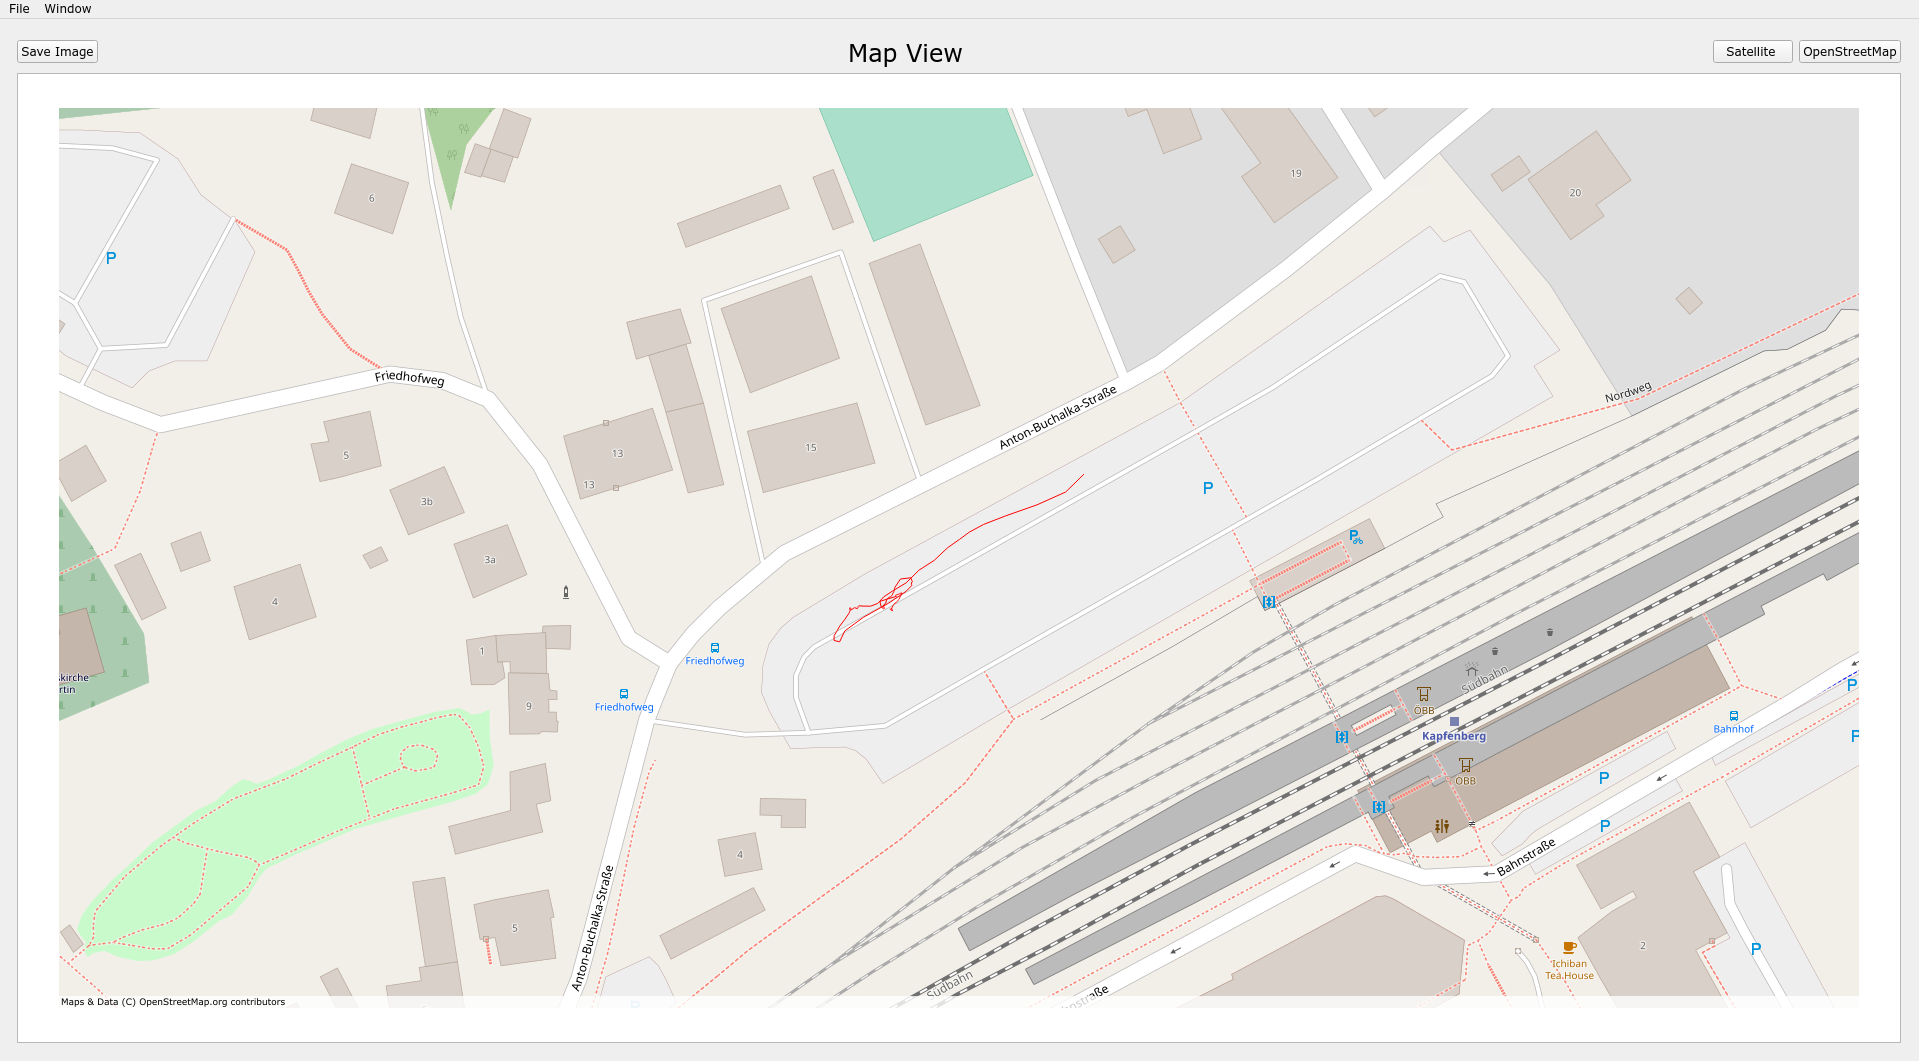
\includegraphics[scale=0.295]{MapViewOSM.png}
\caption{Map View - \ac{OSM}}
\label{fig:OSMMapView}
\end{figure}
\\
Dieselbe Ansicht ist auch als Satellitenbild verfügbar, die Vorgehensweise ist hierbei beinahe ident, anstelle von \ac{OSM} werden die Tiles in diesem Fall von \glqq ArcGISWorldImagery\grqq\ bezogen. Eine solche Karte, ist in Abbildung \ref{fig:SatteliteMapView} ersichtlich. 
\begin{figure}[h]
\centering
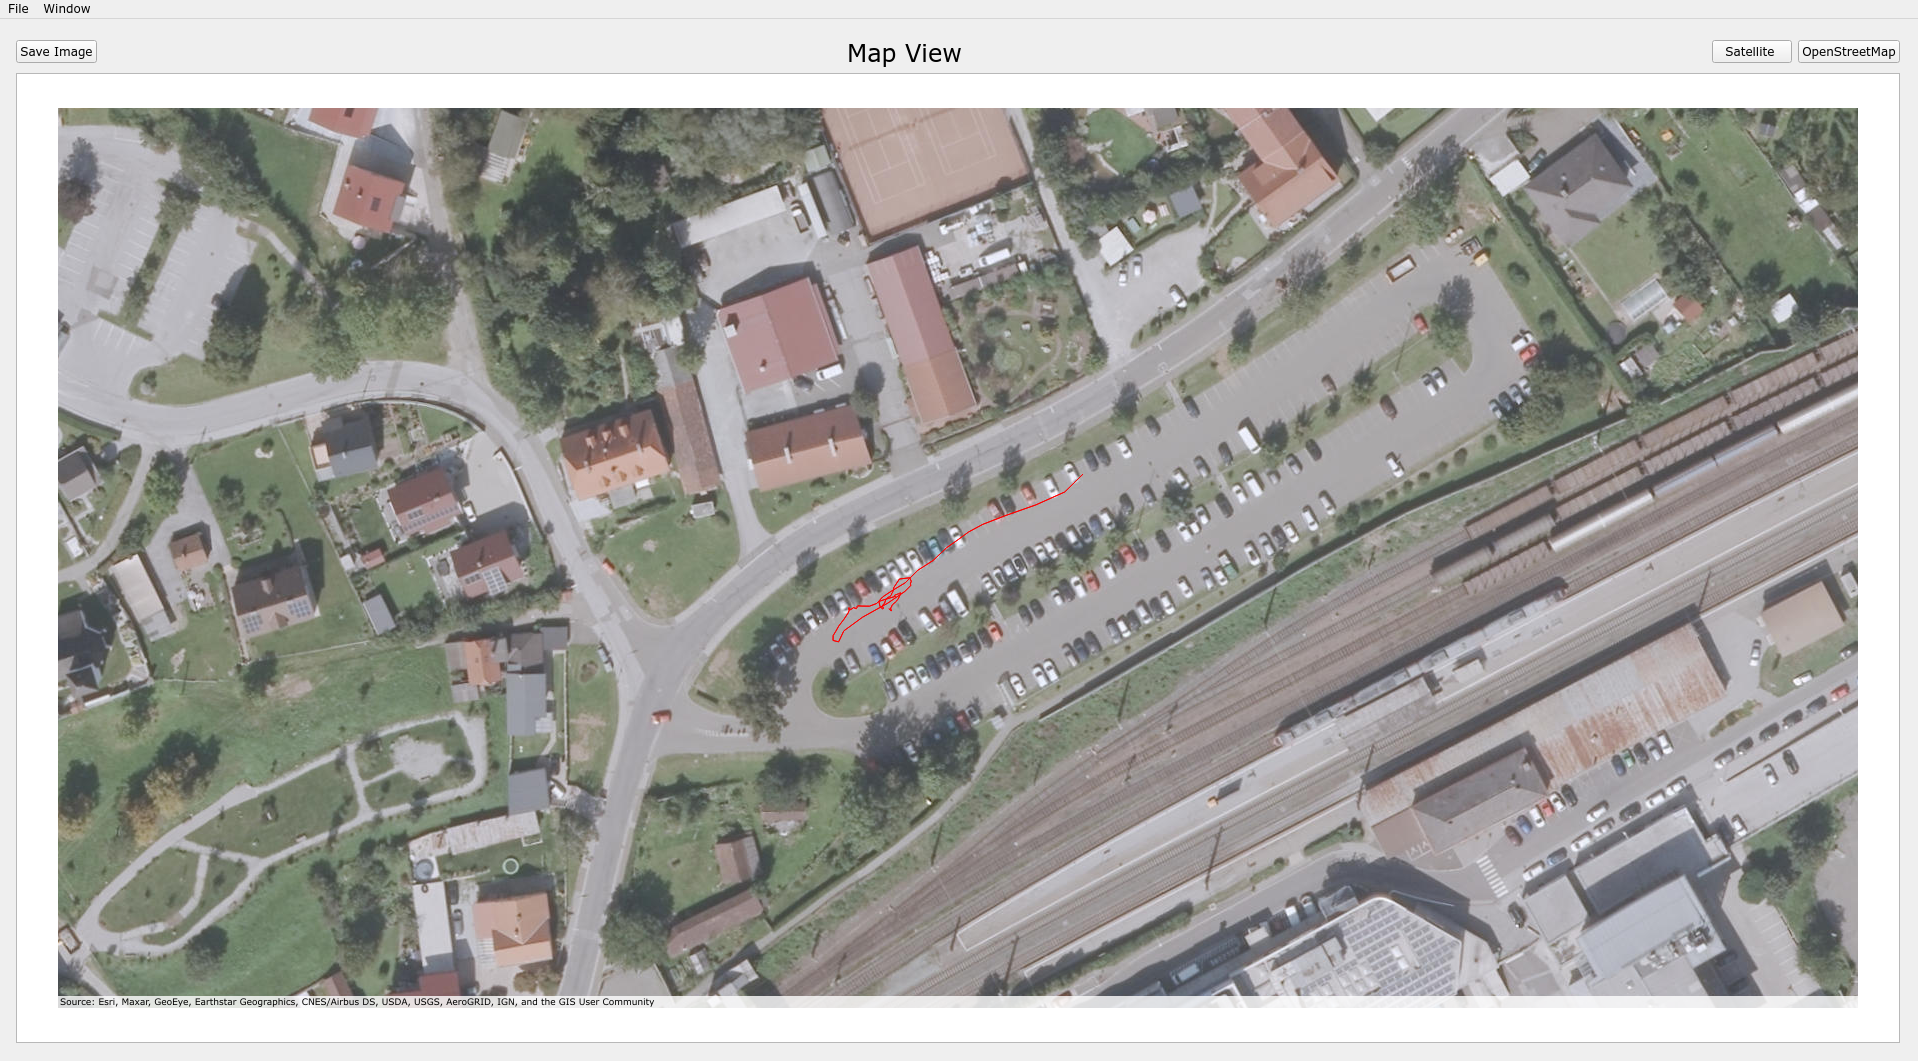
\includegraphics[scale=0.295]{MapViewSatellit.png}
\caption{Map View - Satellitenbild}
\label{fig:SatteliteMapView}
\end{figure}

\subsubsection{Implementation der Map View}
\label{subsubsec:MapViewImplementation}
Diese Ansicht wird mithilfe der in Sektion \ref{subsubsec:tStaticmaps} beschriebenen Python-Bibliothek \glqq py-staticmaps\grqq \ realisiert. Zunächst werden die Koordinaten aus dem Datenset extrahiert, dann werden die einzelnen Punkte miteinander verbunden, um einen Pfad darzustellen. Um den Kartenteil, der heruntergeladen werden soll, festzustellen, wird das Zentrum des Pfades errechnet. Da die Reichweite des ferngesteuerten Autos durch die Sichtweite des Fahrers limitiert ist, kann immer der \ac{OSM}-Zoomfaktor 19 für die Karte verwendet werden. Dieses Kartenstück wird von OpenStreetMap heruntergeladen und mithilfe des Qt-Widgets \glqq QGraphicsView\grqq\ angezeigt.
\newpage
\section{Zusammenfassung}
\label{sec:zusammenfassung}
\newpage
\printbibliography
\newpage
\listoffigures
\newpage
\listoftables
\newpage
\section{Abkürzungsverzeichnis}
\label{sec:Abkuerzungsverzeichnis}

\begin{acronym}
\acro{GPS}{Global Positioning System}
\end{acronym}

\begin{acronym}
\acro{IMU}{Inertial measurement unit}
\end{acronym}

\begin{acronym}
\acro{RPM}{Revolutions per minute}
\end{acronym}

\begin{acronym}
\acro{I2C}{Inter-Integrated Circuit}
\end{acronym}

\begin{acronym}
\acro{CAD}{Computer aided design}
\end{acronym}

\begin{acronym}
\acro{Raspi}{Raspberry Pi}
\end{acronym}

\begin{acronym}
\acro{USB}{Universal Serial Bus}
\end{acronym}

\begin{acronym}
\acro{NMEA}{National Marine Electronics Association}
\end{acronym}

\begin{acronym}
\acro{FDM}{Fused Deposition Modeling}
\end{acronym}

\begin{acronym}
\acro{PLA}{Polyactid}
\end{acronym}

\begin{acronym}
\acro{ABS}{Acrylnitril-Butadien-Styrol}
\end{acronym}

\begin{acronym}
\acro{PETG}{Polyethylenterephthalat-Glycol}
\end{acronym}


\end{document}